\documentclass{ieeetj}
\newcommand{\seclogo}{}
\usepackage{cite}
\usepackage{amsmath,amssymb,amsfonts}
\usepackage{listings}
\usepackage{algorithmic}
\usepackage{graphicx,color}
\usepackage{textcomp}
\usepackage{hyperref}
\usepackage{float}
\usepackage[table,xcdraw]{xcolor}
\definecolor{blau}{RGB}{198, 220, 255} 
\definecolor{gris}{RGB}{176, 176, 176}
\definecolor{verd}{RGB}{ 173, 240, 199}

\hypersetup{hidelinks=true}
\usepackage{algorithm,algorithmic}
\lstset{
    language=Java,
    basicstyle=\ttfamily\small,
    keywordstyle=\bfseries\color{blue},
    stringstyle=\color{red},
    morecomment=[l][\color{magenta}]{//},
    frame=single,
    breaklines=true,
    showstringspaces=false,
    tabsize=1,
}
\def\BibTeX{{\rm B\kern-.05em{\sc i\kern-.025em b}\kern-.08em
    T\kern-.1667em\lower.7ex\hbox{E}\kern-.125emX}}
\AtBeginDocument{\definecolor{tmlcncolor}{cmyk}{0.93,0.59,0.15,0.02}\definecolor{NavyBlue}{RGB}{0,86,125}}

% Definim el logo
\def\OJlogo{
    \vspace{-14pt} % Espai negatiu per pujar el logo
    
\includegraphics[height=0.96cm]{png/logo.png}}

\begin{document}
\receiveddate{08 Maig, 2025}
\publisheddate{09 Juny, 2025}
\currentdate{09 Juny, 2025}

\title{Ramificació i poda: Problema del viatjant de comerç}

\author{Josep Ferriol, Daniel García, Khaoula Ikkene, Biel Perelló} \affil{Universitat de les Illes Balears, Departament d'Enginyeria Informàtica} \corresp{Autor de contacte: Daniel García (email: daniel.garcia19@estudiant.uib.es)}



\begin{abstract}
Aquesta pràctica presenta la resolució del problema del viatjant de comerç (TSP)\cite{TSP} mitjançant un algoritme de tipus \textit{Branch and Bound}, aplicat sobre una representació matricial del graf. S'ha implementat una aplicació en Java que permet visualitzar el procés de cerca de manera interactiva, integrant una arquitectura basada en el patró Model-Vista-Controlador. L'usuari pot modificar la matriu de costos, executar el càlcul de la ruta òptima, i observar els valors clau com el cost total, les branques explorades o els nodes descartats, així com un registre de l'execució. El sistema permet explorar l'eficiència de la poda i els avantatges de la reducció de matrius com a tècnica d'acotació. Es posa èmfasi en la claredat de la visualització gràfica del recorregut i en la modularitat del disseny, fet que facilita tant la comprensió de l’algoritme com la seva extensió futura.
\end{abstract}


\begin{IEEEkeywords}
Problema del viatjant de comerç, TSP, reducció de matrius, graf dirigit i amb pesos, matriu d'adjacència, cost computacional, model-vista-controlador, inferfície gràfica, GUI, arquitectura
\end{IEEEkeywords}


\maketitle


\section{Introducció}
El problema del viatjant de comerç (TSP, per les seves sigles en anglès Travelling Salesman Problem)\cite{TSP} és un dels problemes més clàssics i estudiats en l'àmbit de l'optimització combinatòria i la teoria de la complexitat computacional. El seu enunciat és aparentment senzill:\textbf{ donada una llista de ciutats i les distàncies entre cada parell, quin és el recorregut més curt que permet visitar totes les ciutats exactament una vegada i tornar a la ciutat d’origen?} Malgrat la seva simplicitat, es tracta d’un problema \textit{NP-dur\cite{NP-hard}}, fet que implica que no es coneix cap algoritme eficient que el resolgui de manera òptima per a tots els casos, especialment quan el nombre de ciutats creix.\newline

El TSP és important tant des del punt de vista teòric com pràctic. Ha estat utilitzat com a problema de referència per desenvolupar i provar mètodes d’optimització, ja que encapsula molts dels reptes típics de la cerca d’una solució òptima en espais de solucions molt grans. 
Tot i la seva dificultat, existeixen nombrosos algorismes exactes i heurístics que permeten resoldre instàncies de mida considerable, arribant a desenes de milers de ciutats en casos resolts exactament i milions en aproximacions molt precises.\newline

Les aplicacions del TSP\cite{aplicacions-TSP} són diverses i sovint sorprenents: des de la planificació de rutes logístiques, la fabricació de microxips, o la seqüència d’ADN, fins a la programació de l’observació astronòmica, on cal minimitzar el temps de moviment del telescopi entre fonts d’interès. A més, el TSP es pot generalitzar en problemes com el problema del comprador viatger\cite{comprador-viatjer}, el vehicle routing problem\cite{routing-problem} o el ring star problem\cite{ring-star-problem}, que introdueixen restriccions addicionals com recursos limitats o finestres de temps. Així doncs, el TSP és molt més que un simple trencaclosques: és una eina fonamental per entendre i resoldre problemes reals de gran complexitat.


\section{Marc teòric} 
En aquest apartat es descriuen els fonaments teòrics necessaris per entendre el projecte, abastant des de conceptes relacionats amb la gestió de grafs  fins a aspectes d’arquitectura de programari i execució concurrent a Java.

\subsection{Ramificació i poda}
La Ramificació i Poda (Branch and Bound, o B\&B)\cite{BB} és una tècnica que es pot considerar com una extensió o millora dels algorismes de \textbf{Backtracking}. El seu objectiu principal és optimitzar la cerca en un arbre de possibilitats reduint-ne la mida mitjançant una \textit{heurística o criteri intel·ligent}. 
Aquesta tècnica és especialment útil en problemes d’optimització, on es poden aplicar restriccions per eliminar camins no prometedors. \newline

La poda del arbre es realitza descartant rames que no poden conduir a una solució millor que la millor trobada fins al moment. Això es fa utilitzant una \textbf{cota}, que s’estima per a cada node; si aquesta cota és pitjor que la millor solució actual, es descarta la branca. Això permet reduir dràsticament el nombre de nodes explorats, superant l’eficiència dels algoritmes de \textbf{Backtracking} que solen tenir un creixement factorial o exponencial.\newline

Finalment, l’exploració de l’arbre es pot dur a terme amb diverses estratègies, com ara \textbf{en profunditat (LIFO)}, \textbf{en amplada (FIFO)} o \textbf{seleccionant el node més prometedor mitjançant una estructura de monticle (heap)}.\newline

L'algorisme general es pot descriure de la següent manera.
\begin{enumerate}
  \item Segons l'estratègia, se selecciona el node que s'explorarà.
  \item Es generen les branques corresponents a aquest node.
  \item Per a cada nou node, es calcula una estimació (cota) del valor més prometedor.
  \item Es poden les branques que no poden superar la millor solució coneguda.
\end{enumerate}

\subsection{Reducció de matrius}

La \textbf{reducció de matrius}\cite{reduccio-matrius} és una tècnica fonamental utilitzada en l’algorisme de Ramificació i Poda per resoldre problemes com el del Viatjant de Comerç (TSP). 
Aquesta tècnica consisteix a transformar la matriu de costos inicial (matriu d'adjacència) reduint cada fila i columna per tal que el valor mínim de cadascuna sigui zero. Aquesta operació no altera la solució òptima del problema, però permet establir una \textit{cota inferior} inicial que s’utilitza per decidir si una branca pot ser descartada (poda). Quan es fa una selecció d’una aresta en el camí del TSP, s’actualitza la matriu (eliminant files i columnes corresponents i bloquejant cicles prematurs) i es repeteix el procés de reducció per obtenir noves cotes. Aquest procés és clau per millorar l’eficiència computacional, ja que permet evitar l’exploració de gran part de l’arbre de possibilitats.

\subsection{Problema del viatjant de comerç}

Tal com s'ha detallat en la secció d'introducció, el problema del viatjant de comerç (TSP) és un problema clàssic en l'àmbit de l'optimització combinatòria, àmpliament estudiat per la seva simplicitat d'enunciat i la seva gran varietat d'aplicacions pràctiques, com ara la planificació de rutes, la logística o la fabricació de circuits. L'enunciat del problema consisteix a trobar el recorregut més curt que permet visitar un conjunt de ciutats exactament una vegada cadascuna i tornar al punt d'origen.\newline

Aquest problema es pot representar tant de manera visual com matemàtica. Visualment, es modela com un graf dirigit o no dirigit amb pesos, on els nodes representen les ciutats i les arestes representen les distàncies (o costos) entre elles. Matemàticament, aquesta mateixa informació es pot expressar mitjançant una matriu d’adjacència, on cada element $(i,j)$ conté la distància o cost de viatjar de la ciutat $i$ a la ciutat $j$. \newline

Quan s’aplica el mètode de ramificació i poda per resoldre el TSP, el problema es transforma en una sèrie de càlculs matricials. Aquests càlculs inclouen la reducció de la matriu de costos per obtenir una cota inferior inicial, i l'actualització d’aquesta matriu en cada pas de la ramificació, a mesura que es van seleccionant camins i es descarten branques que no poden conduir a una solució òptima. Aquesta aproximació, tot i ser computacionalment costosa, permet optimitzar l’exploració de solucions i evitar l’exploració exhaustiva de totes les permutacions possibles.



\subsection{Concurrència i Model d’Execució en Java}


\section{Entorn de Programació}

Per dur a terme el desenvolupament d’aquesta pràctica, s’ha utilitzat un conjunt d’eines i tecnologies que han proporcionat un entorn robust i eficient. A continuació es detallen les eines principals emprades:

\begin{itemize}
    \item \textbf{Llenguatge de programació: Java} – El projecte s’ha desenvolupat íntegrament en Java. Java és un llenguatge de programació orientat a objectes reconegut per la seva estabilitat, portabilitat i àmplia col·lecció de llibreries estàndard. L’ús de Java ha permès escriure codi mantenible i independent de la plataforma, executant-se sobre la màquina virtual Java (JVM) en diversos sistemes operatius sense modificacions.\newline

    \item \textbf{Interfície gràfica: Swing} – S’ha emprat la llibreria gràfica Swing (part del JDK de Java) per construir la interfície d’usuari de l’aplicació. Swing proporciona un conjunt complet de components GUI (botons, finestres, menús, taules, etc.) amb altes capacitats de personalització i maneig d’esdeveniments \cite{SwingLibrary}. A més, la seva arquitectura segueix el patró MVC, la qual cosa s’alinea amb el disseny de l’aplicació\cite{MVC_Theory}. Mitjançant Swing s’ha implementat una vista interactiva on l’usuari pot triar els idiomes a comparar, iniciar i cancel·lar anàlisis i visualitzar els resultats (per exemple, mostrant percentatges de similitud).\newline

    \item \textbf{Entorn de desenvolupament: IntelliJ IDEA} – S’ha utilitzat l’entorn de desenvolupament integrat (IDE) IntelliJ IDEA per escriure i organitzar el codi Java. IntelliJ proporciona funcionalitats avançades com l’autocompleció intel·ligent del codi, la detecció d’errors en temps real, eines de refactorització i una integració fluïda amb sistemes de control de versions com Git. Aquestes característiques han facilitat la codificació i depuració del projecte, contribuint a un desenvolupament més àgil i menys propens a errors.\newline

    \item \textbf{Control de versions: Git i GitHub} – Per gestionar el codi font i portar un seguiment de l’evolució del projecte, s’ha emprat Git com a sistema de control de versions. El codi s’ha allotjat en un repositori privat a GitHub, la qual cosa ha permès la col·laboració entre els integrants de l’equip i ha garantit un historial de canvis ben documentat. Gràcies a Git s’han pogut integrar noves funcionalitats i corregir errors de manera controlada, i revertir canvis si calia, assegurant l’estabilitat del codi al llarg del desenvolupament.\newline

    \item \textbf{Plataforma de documentació: Overleaf} – La memòria tècnica del projecte (el present document) s’ha redactat utilitzant LaTeX mitjançant la plataforma en línia Overleaf. \newline Aquesta plataforma ha facilitat l’edició col·laborativa del text, el control de versions de la documentació i la utilització de la plantilla IEEE proporcionada, incloent-hi la inserció del logotip i el format requerit. \newline
    L’ús de LaTeX ha assegurat una presentació professional del document, amb una gestió senzilla de les citacions bibliogràfiques i la numeració automàtica de seccions, figures i taules.
\end{itemize}

L’elecció d’aquest conjunt d’eines ha permès garantir un desenvolupament estructurat i eficient del projecte. Java i Swing han proporcionat el nucli tecnològic per implementar la funcionalitat i la interfície, mentre que IntelliJ ha accelerat el flux de treball de codificació. GitHub ha assegurat una correcta coordinació del treball en equip, i Overleaf ha contribuït a documentar de manera clara i organitzada tot el procés de desenvolupament.



\section{Desenvolupament i Metodologia}




\subsection{Arquitectura general del sistema}
El projecte s'ha estructurat seguint el patró \textbf{Model–Vista–Controlador (MVC)}, que permet una clara separació de responsabilitats:
\begin{itemize}
    \item \textbf{Model}: La interfície \texttt{Comunicar.Java} juntament amb la classe principal del programa \texttt{Main.java} són els responsables d'establir la comunicació i alinear les parts del programa per poder comunicar les peticions de l'usuari, executar l'algorisme corresponent i mostrar els resultats obtinguts.
    
    \item \textbf{Vista}: Implementada amb Swing, proporciona una interfície gràfica intuïtiva i flexible per a la interacció amb l'usuari. 

\item \textbf{Controlador}: Actua com a intermediari, processant els esdeveniments de la GUI i invocant accions sobre el \textbf{Model}, a través de la interfície \textit{Comunicar} i la classe \textit{Main.java}.
\end{itemize}


\subsection{Estructura de paquets i classes}
L'estructura del programa segueix les bones pràctiques d'encapsulament de Java. 
Els paquets principals es poden identificar d'acord amb el disseny de l'arquitectura Model-Vista-Controlador. 
La figura següent il·lustra l'estructura del nostre programa. \newline
Els quadres de colors representen diferents elements: \textcolor{blau}{els blaus}, les \textbf{classes}; \textcolor{gris}{els grisos}, les \textbf{interfícies};\textcolor{verd}{ i els altres}, els \textbf{paquets}.

\begin{figure}[H]
    \centering
    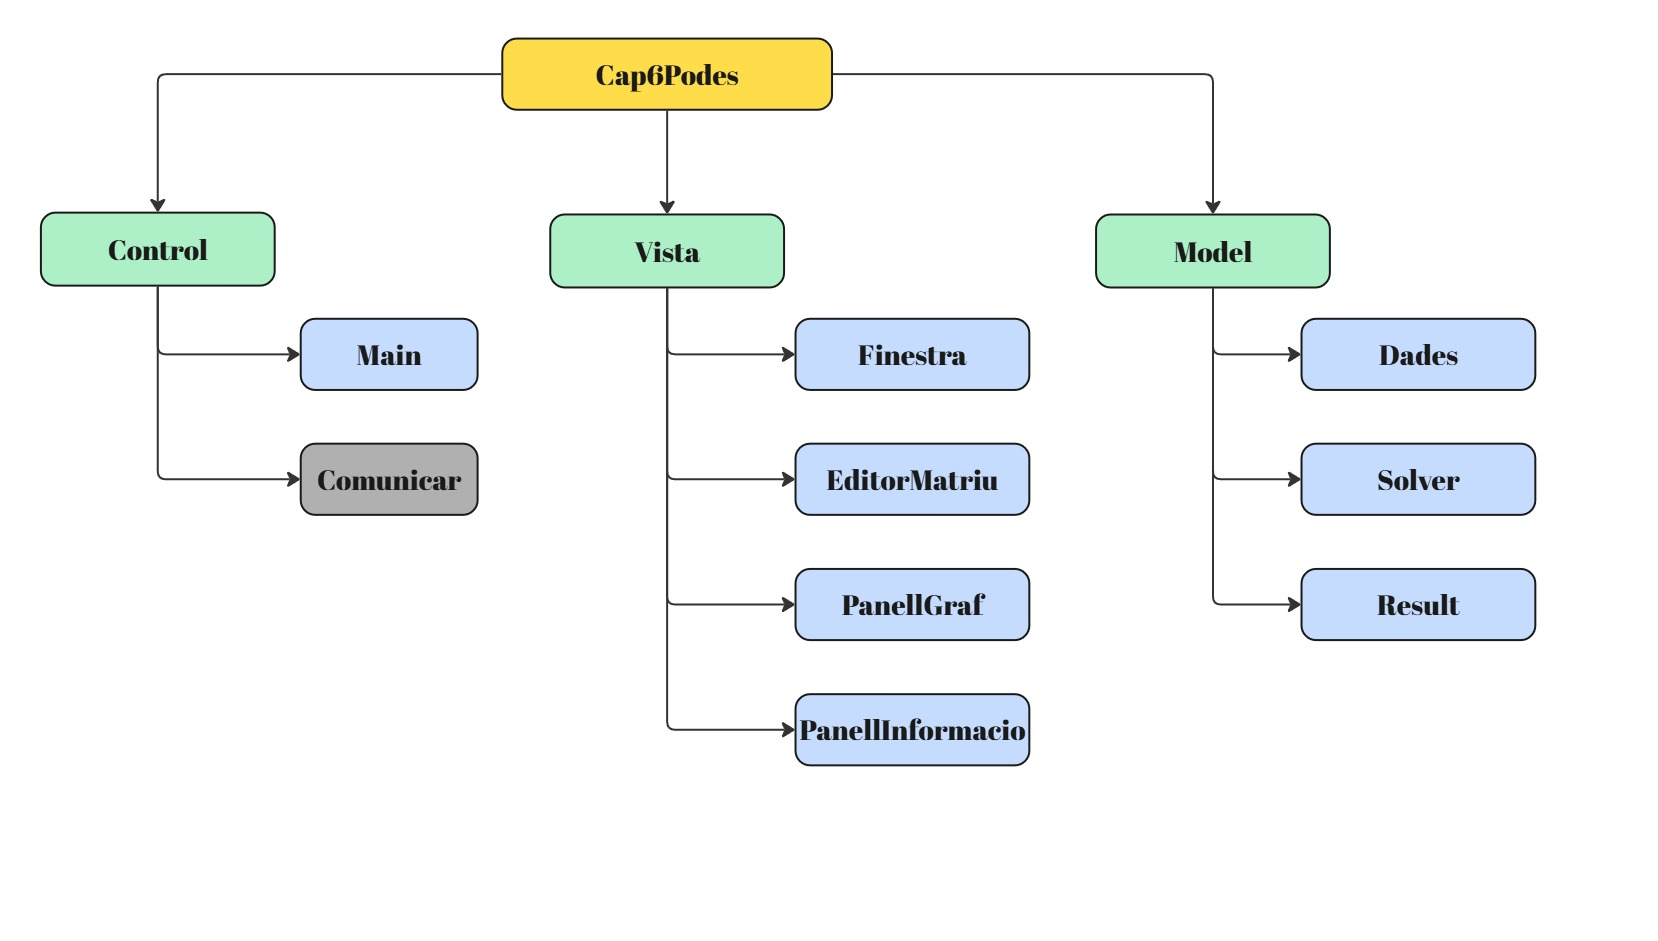
\includegraphics[width=0.45\textwidth]{png/estructura.jpg}
    \caption{Estructura de paquets i classes }
    \label{fig:enter-label}
\end{figure}

\subsection{Algorisme del viatjant de comerç} 
La classe principal que encapsula l’algorisme per a la resolució del problema del viatjant de comerç és \texttt{Solver.java}.

Atès que el problema consisteix a recórrer un graf dirigit, l’estructura més adequada per emmagatzemar la informació necessària són els nodes. És per això que s’ha creat una classe específica on es guarden diversos atributs que permeten construir el recorregut òptim sol·licitat.

\begin{lstlisting}[language = JAVA, breaklines = true]
public static class Node implements Comparable<Node> {
    int[][] matriuReduida;
    int actual; //vertex del node actual
    int cost;  //cost acumulat fins el node actual
    Node pare;
    int profund;

    Node(int[][] reducedMatrix, int actual, int cost, Node pare, int profund)   {
        this.matriuReduida = reducedMatrix;
        this.actual = actual;
        this.cost = cost;
        this.pare = pare;
        this.profund = profund;
        }
@Override
public int compareTo(Node o) {
    return Integer.compare(this.cost, o.cost);
    }
}
\end{lstlisting}

L'algorisme implementa la selecció del node més prometedor mitjançant una \textit{PriorityQueue} que manté els nodes ordenats segons el seu cost acumulat, seguint l'estratègia de \textit{Branch-and-Bound}.\newline

Inicialment, es crea el node arrel, \textit{root}, que correspon a la primera ciutat —concretament, la primera ciutat de la matriu—, i se'n calcula el cost de reducció per obtenir una primera estimació del mínim possible. \newline


A mesura que hi ha nodes per explorar i encara no s'han visitat totes les ciutats, s'extreu el node de menor cost de la cua de prioritats, es processa i es generen els seus nodes fills. Per a cada node extret, es verifica si totes les ciutats han estat visitades (\textit{depth == totalNodes - 1}), cas en el qual s'afegeix el cost de retorn i es retorna com a solució òptima. Si encara hi ha ciutats disponibles, es generen nous nodes fills marcant com a \textit{INFINITY} les connexions ja visitades, es recalcula el cost acumulat i el cost de reducció, i els nous nodes s'insereixen a la \textit{PriorityQueue} per continuar l'exploració en ordre de menor cost.

S'utilitzen varies mètodes auxiliars per al bon funcionament de l'algorisme, en comentarem els següents.

\begin{lstlisting} [language = JAVA, breaklines = true]
private Node crearNodeFill(Node parent, int nextVertex) {
    int[][] matriu = deepCopy(parent.matriuReduida);
    int current = parent.actual; 
    // Marcar fila i columna amb INFINTY per eliminar camins ja visitats.
    for (int k = 0; k < totalNodes; k++) {
        matriu[current][k] = INFINITY;
        matriu[k][nextVertex] = INFINITY;
    }
    int costAfegit = parent.matriuReduida[current][nextVertex];
    int costReduccio = calcularCostReduccio(matriu);
    return new Node(matriu, nextVertex, parent.cost + costAfegit + costReduccio, parent, parent.profund + 1);
    }    
\end{lstlisting}
El mètode \texttt{crearNodeFill} genera un nou node fill a partir d'un node pare, aplicant una estratègia de creació basada en la còpia i la modificació de la matriu de costos reduïda. \newline
Inicialment, es fa una còpia profunda de la matriu del node pare per garantir que les modificacions no afectin el node original.\newline 

A continuació, es procedeix a marcar la fila i la columna corresponents al node actual i al nou node (\textit{nextVertex}) amb valors d'\textit{INFINITY}, eliminant així les connexions ja visitades i evitant que es repeteixin ciutats en el recorregut.\newline

Un cop ajustada la matriu, es calcula el cost afegit del moviment des del node actual fins al nou node, basant-se en la matriu original del node pare. 

Posteriorment, es recalcula el cost de reducció de la matriu modificada per obtenir un valor heurístic que permet ajustar l'exploració cap a solucions més prometedores. 
Finalment, es crea un nou objecte \texttt{Node} que incorpora la nova matriu, el node destí, el cost acumulat i la profunditat incrementada, assegurant que el procés de generació de fills manté la coherència i la progressió dins l'algorisme de \textit{Branch-and-Bound}.


\begin{lstlisting}[language = JAVA, breaklines = true]
private int calcularCostReduccio(int[][] mat) {
    int cost = 0;
    // reduir files
    for (int i = 0; i < mat.length; i++) {
        int minFila = trobarMinFila(mat, i);
        if (minFila != INFINITY) {
            cost += minFila;
            for (int j = 0; j < mat.length; j++) {
                if (mat[i][j] != INFINITY) {
                    mat[i][j] -= minFila;
                    }
                }
            }
    }
     //reduir columnes
    for (int i = 0; i < mat.length; i++) {
        int minColumna = trobatMinColumna(mat, i);
        if (minColumna != INFINITY) {
            cost += minColumna;
            for (int j = 0; j < mat.length; j++) {
                if (mat[j][i] != INFINITY) {
                    mat[j][i] -= minColumna;
                    }
                }
            }
        }
        return cost;
    }    
\end{lstlisting}

El mètode \texttt{calcularCostReduccio} redueix la matriu de costos per obtenir una estimació del cost mínim necessari per completar el recorregut. Primer, recorre cada fila, troba el valor mínim i el resta de tots els elements de la fila, acumulant aquest valor en el cost total. 

Posteriorment, s’aplica el mateix procediment a les columnes, i el cost obtingut de la seva reducció s’afegeix al cost total.

La reducció, com s'ha comentant prèviament, garanteix que la matriu obtinguda tingui almenys un zero per fila i columna, ajudant a la \textbf{poda} en l'algorisme de \textit{Ramificació i poda}.


\medskip
\noindent

\subsection{Gestió de concurrència}
La gestió de la concurrència es realitza amb \texttt{ExecutorService}. Gràcies a l’ús d’aquest executor, es disposa d’un control dels fils simultanis mitjançant una cua d’espera.

Però s'ha de tenir en compte, que degut a la naturalesa iterativa del algorisme implementat, no es pot fer de forma concurrent. no obstant sí es manté en fils separats tant la vista com el controlador, a més dels processos del model com es costum en les nostres pràctiques.

\subsection{Visualització i interacció amb l'usuari}

La interfície gràfica d’usuari (GUI) s’ha desenvolupat utilitzant la llibreria \texttt{Swing} de Java, adoptant una arquitectura basada en el patró Model-Vista-Controlador (MVC)\cite{mvcPattern}. Aquesta separació de responsabilitats ha permès un desenvolupament modular i facilita tant la reutilització com el manteniment del codi. El disseny de la vista s’ha centrat en proporcionar una representació clara i eficaç del graf, tot preservant l’escalabilitat davant diferents grandàries d’instàncies.

\paragraph{Estructura principal de la Finestra.}
La classe \texttt{Finestra} representa el contenidor principal de la GUI, és a dir, la finestra principal de l’aplicació. Estén la classe \texttt{JFrame} i integra tots els components de la interfície: el panell de botons de control (amb accions per calcular o editar la matriu), el panell de visualització gràfica, i el panell lateral d’informació. La finestra inicialitza aquests components i en gestiona la disposició mitjançant un \texttt{BorderLayout}. A més, implementa la interfície \texttt{Comunicar}, que permet a altres parts del sistema (especialment el controlador) notificar actualitzacions visuals com la necessitat de repintar el gràfic. També inclou un \texttt{JCheckBox} que activa la visualització per passes del programa\newline

El component principal de la visualització és el \texttt{PanellGraf}, una subclasse de \texttt{JPanel}, encarregada de representar visualment els nodes i les arestes del graf dirigit i ponderat. Aquesta classe gestiona internament el procés de dibuix mitjançant la redefinició del mètode \texttt{paintComponent}, aprofitant les capacitats de la classe \texttt{Graphics2D} per a oferir un control precís sobre el traçat vectorial de formes, textos i línies.\newline

\begin{figure}[H]
    \centering
    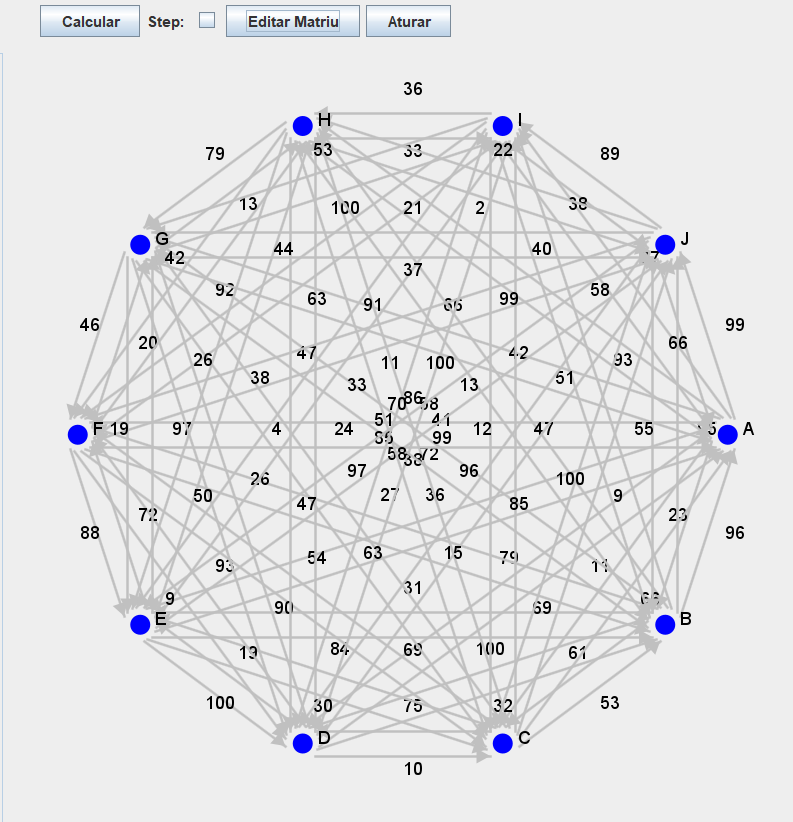
\includegraphics[width=0.45\textwidth]{png/graf.png}
    \caption{Panell Graf}
\end{figure}

Per tal d’assegurar una representació visual adaptativa, s’ha implementat un mètode intern anomenat \texttt{ajustarParametresVisuals}, el qual modifica dinàmicament paràmetres com el radi de disposició dels nodes, la mida de les fletxes, la separació de les etiquetes i la mida de la font, en funció del nombre de nodes del graf i de les dimensions actuals del panell. Aquest ajust automàtic permet visualitzar grafs de mida mitjana i gran sense que es produeixin solapaments innecessaris ni que els elements gràfics excedeixin els límits visibles del panell.\newline

Els nodes del graf es distribueixen seguint una disposició circular, equiespaiada en angle respecte al centre del panell. Aquesta estratègia geomètrica garanteix una distribució regular independentment de la mida del graf. Cada node es representa com un cercle ple de color blau amb una lletra identificativa (A, B, C, etc.) situada en posició relativa.\newline

Pel que fa a les arestes, s’han tingut en compte tant les connexions unidireccionals com les bidireccionals. Per evitar el solapament de les fletxes entre parelles de nodes amb arestes en ambdues direccions (i possiblement pesos diferents), s’ha implementat una tècnica de desplaçament perpendicular sobre el vector d’unió. Aquesta tècnica permet desviar lleugerament una de les fletxes, mantenint-ne la llegibilitat i evitant confusions visuals. Els pesos associats a les arestes es mostren al llarg de la línia corresponent, desplaçats lleugerament en una direcció perpendicular per evitar que se superposin amb el traçat de la fletxa.\newline

L’estructura del panell permet una fàcil integració dins una finestra principal que inclou, entre altres elements, panells addicionals per a la selecció de fitxers, l’execució d’algorismes, i la visualització de resultats. Aquesta arquitectura modular es reflecteix en l’existència de diversos panells especialitzats (\texttt{PanellGraf}, \texttt{EditorMatriu},  \texttt{PanellInformació}  etc.), cadascun responsable d’una part concreta de la interacció amb l’usuari, afavorint així la separació de preocupacions.

\paragraph{PanellInformacio.}
Aquest component estàtic de la interfície actua com a panell informatiu del procés de resolució i té com a objectiu proporcionar a l’usuari dades rellevants de l’execució de l’algorisme \textit{Ramificació i poda}. Mostra valors com el cost total de la millor solució trobada, el nombre de branques explorades, el nombre de nodes descartats i una estimació de l'eficiència de la poda mitjançant una mètrica personalitzada. També incorpora una àrea de text amb barres de desplaçament on es registren missatges informatius generats durant l’execució, fent funcions de log simplificat. 
La seva implementació s’ha resolt emprant components de la llibreria \texttt{Swing}, amb un disseny vertical mitjançant \texttt{GridLayout} i distribució \texttt{BorderLayout} global.

\begin{figure}[H]
    \centering
    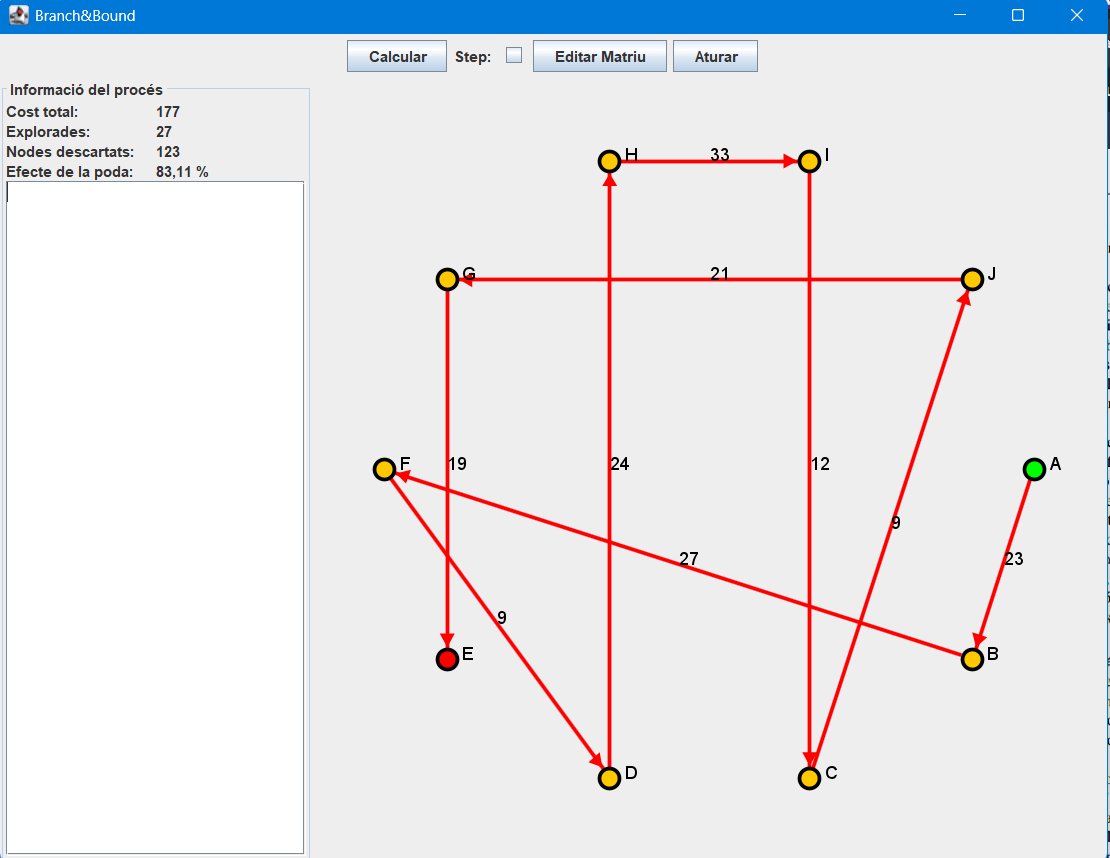
\includegraphics[width=0.45\textwidth]{png/finestra.png}
    \caption{Exemple de la finestra completa }
    \label{fig:enter-label}
\end{figure}

\paragraph{EditorMatriu.}
El diàleg \texttt{EditorMatriu} permet a l’usuari editar la matriu de costos del graf manualment o generar-ne una de nova aleatòriament. Es presenta com una finestra modal, amb una taula editable on cada cel·la representa el cost d’un arc entre dos nodes. També incorpora camps de configuració per establir les dimensions del graf i un conjunt de botons per aplicar els canvis o generar noves dades. 
Aquesta eina resulta especialment útil en fase de proves, ja que facilita la manipulació directa de l’estructura de dades principal del model sense haver de modificar el codi font o recórrer a fitxers externs, tot i què permet la importació i exportació de la matriu d'adjacència des d'arxius CSV\newline

La interacció principal amb el panell de graf es realitza de forma passiva, mostrant la informació de manera immediata en carregar un graf. La interfície ha estat dissenyada per facilitar possibles ampliacions futures que podrien incloure funcionalitats interactives com la selecció de nodes, l’execució dinàmica d’algorismes sobre el graf o la modificació directa de connexions.\newline

En definitiva, la vista desenvolupada proporciona una representació clara, escalable i coherent del graf, permetent a l’usuari interpretar-ne fàcilment l’estructura i els pesos, alhora que prepara el terreny per a futures millores interactives i d’usabilitat.

\begin{figure}[H]
    \centering
    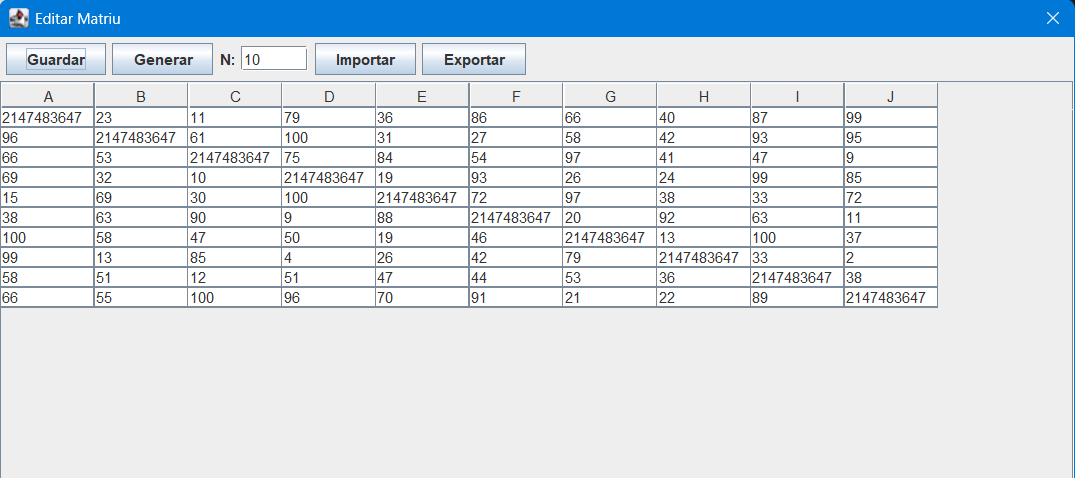
\includegraphics[width=0.45\textwidth]{png/matriu.png}
    \caption{Editor de matriu}
    \label{fig:enter-label}
\end{figure}

\subsection{Decisions de disseny i extres implementats}
Pel que fa a les funcionalitats extres, se n’han implementat diverses. En primer lloc, la matriu d’adjacència es pot generar automàticament i de forma aleatòria introduint un valor \textbf{N}, que indica la dimensió o el nombre de ciutats que ha de tenir el graf. Aquesta matriu també es pot modificar manualment, així com ser importada o exportada en formats \texttt{CSV} o \texttt{TXT}.

Quant al graf del problema, es mostra a la finestra principal juntament amb informació rellevant per entendre el funcionament intern de l’algorisme, com ara el nombre de nodes visitats, els nodes podats, el cost total, entre altres dades, tal com s’indica a l’enunciat de la pràctica.

A més, es permet la visualització progressiva de la solució trobada per al camí òptim. Aquesta funcionalitat es pot activar mitjançant el botó \textbf{Step} situat a la finestra principal.

\section{Resultats i Comparació}
En aquesta secció farem diverses comparacions, segons el temps d'execució, l'ús de memòria.

\begin{table}[H]
\centering
\caption{Temps d'execució en funció de $N$}
\begin{tabular}{|c|c|}
\hline
\textbf{N} & \textbf{Temps d'execució (ms)} \\
\hline
5 & 1 \\
10 & 2 \\
15 & 9 \\
20 & 20 \\
25 & 616 \\
30 & 974 \\
\hline
\end{tabular}
\end{table}

\begin{table}[H]
\centering
\caption{Memòria utilitzada pel Solver}
\begin{tabular}{|c|c|}
\hline
\textbf{N} & \textbf{Memòria utilitzada (KB)} \\
\hline
5 & 0 \\
10 & 285 \\
15 & 20 \\
20 & 58 \\
25 & 80 \\
30 &128 \\
\hline
\end{tabular}
\end{table}
Mostrarem els resultats de forma visual per millor lectura.
\begin{figure}[H]
    \centering
    \includegraphics[width=0.45\textwidth]{png/Temps d'execució segons el nombre de ciutats.png}
    \caption{Temps d'execució segons el nombre de ciutats}
\end{figure}

\begin{figure}[H]
    \centering
    \includegraphics[width=0.45\textwidth]{png/Memòria usada segons el nombre de ciutats.png}
    \caption{Memòria usada segons el nombre de ciutats}
\end{figure}

El temps d'execució sembla raonable per nombres petits de ciutats. A mesura que aquest augmenta, el temps es comporta de manera aparentment lineal. No obstant això, quan s'arriba a més de vint ciutats, es produeix un increment molt més notable del temps d'execució. Amb 30 ciutats, el rendiment es deteriora dràsticament, gairebé arribant a un temps indefinit, ja que l'espai limitat de la heap de Java s'esgota a aquesta escala. El principal problema que origina aquesta limitació resideix en el gran cost que comporta copiar tota la matriu a l'hora de crear cada node fill.\newline

Pel que fa a la memòria, l’ús augmenta bastant entre 5 i 10 ciutats, probablement per l’escalfament inicial de la màquina virtual de Java (JVM). Després d’això, el consum es manté més estable i creix de manera més lenta i gradual, tot i que continua augmentant a mesura que el problema es complica.



\section{Conclusions}

Al llarg d’aquest projecte s’ha abordat la resolució del problema del viatjant de comerç mitjançant la tècnica de ramificació i poda. Aquesta aproximació ha permès reduir l’espai de cerca respecte a una exploració exhaustiva, però també ha evidenciat les seves limitacions quan s’incrementa la mida del problema.

L’anàlisi empírica dels resultats ha demostrat que, tot i que l’algorisme és eficient per a instàncies amb un nombre reduït de ciutats, el seu rendiment es degrada notablement a partir de 20 ciutats. Aquest comportament es deu principalment a la complexitat inherent del problema, però també a decisions d’implementació com la còpia recurrent de la matriu de distàncies per a cada node fill, que incrementa considerablement l’ús de memòria i temps d’execució.

A més, s’ha observat que el consum de memòria no és del tot lineal, i que factors com l'escalfament inicial de la màquina virtual de Java poden tenir un impacte significatiu en les primeres execucions. No obstant això, la memòria tendeix a estabilitzar-se per valors moderats de $N$ abans d’incrementar-se novament en instàncies més grans.

També cal destacar la complexitat associada a la representació gràfica del graf dirigit a la finestra. Tot i que el dibuix de ciutats i connexions entre elles pot semblar trivial, la gestió correcta de les coordenades, l’escalat, l’orientació de les fletxes i l’etiquetatge de pesos implica una càrrega computacional i algorísmica significativa, especialment quan el nombre de ciutats creix. Cal tenir en compte que la representació visual ha de ser clara, llegible i eficient, evitant la superposició d’elements i assegurant la responsivitat de la interfície gràfica. Per aquest motiu, l’eficiència del codi de visualització i la separació clara de responsabilitats dins el patró Model-Vista-Controlador han estat fonamentals per garantir una experiència d’usuari fluida.


En definitiva, aquest treball ha permès entendre les fortaleses i febleses de la tècnica de ramificació i poda aplicada a problemes NP-complets. Tot i ser una alternativa més eficient que la cerca exhaustiva, és essencial acompanyar-la d’optimitzacions addicionals (com l’ús de heurístiques, estructures de dades més eficients o millores en la gestió de memòria) per tal de garantir-ne l’escalabilitat i aplicabilitat a problemes de major dimensió.

\medskip

\noindent
\textbf{Valoració personal de l'equip:} La realització d’aquest projecte ens ha permès aprofundir tant en aspectes teòrics com pràctics dels algorismes de cerca i optimització. Hem après a gestionar de manera rigorosa l’eficiència computacional, a identificar colls d’ampolla en la implementació, i a extreure conclusions rellevants a partir dels resultats experimentals. A més, aquest treball ens ha ajudat a consolidar la importància d’una bona planificació, així com de la col·laboració i la comunicació dins d’un equip, factors clau per a l’èxit en projectes d’enginyeria informàtica.



\begin{figure}[H]
    \centering
    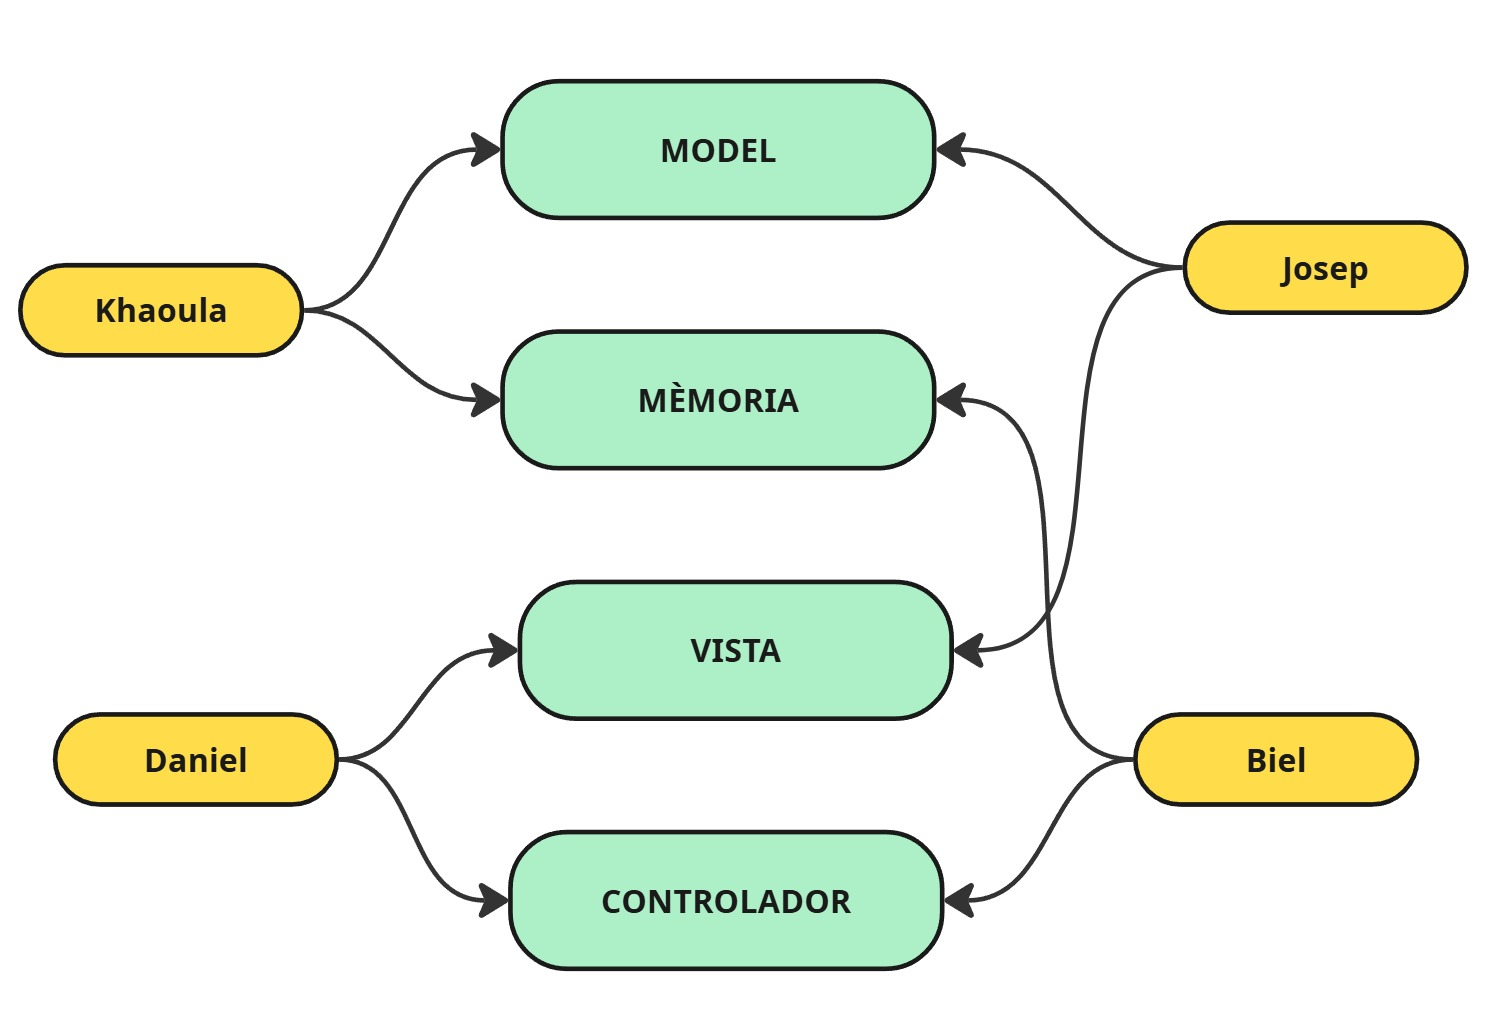
\includegraphics[width=0.45\textwidth]{png/repartiment.jpg}
    \caption{Repartiment de tasques}
    \label{fig:enter-label}
\end{figure}

\bibliographystyle{plain}
\begin{thebibliography}{9}
\bibitem{TSP}
Wikipedia, \textit{Travelling Salesman Problem}, Wikipedia Foundation, 2024. \\
\url{https://en.wikipedia.org/wiki/Travelling_salesman_problem}.

\bibitem{BB}
GeeksforGeeks, \textit{Branch and Bound Algorithm}, GeeksforGeeks, 2024. \\
\url{https://www.geeksforgeeks.org/branch-and-bound-algorithm/}.

\bibitem{NP-hard}
Wikipedia, \textit{NP-hardness}, Wikipedia Foundation, 2024. \\
\url{https://en.wikipedia.org/wiki/NP-hardness}.

\bibitem{aplicacions-TSP}
Wikipedia. (s.f.). \textit{Travelling salesman problem}.\\
\url{https://en.wikipedia.org/wiki/Travelling_salesman_problem#:~:text=The%20TSP%20has%20several%20applications,areas%2C%20such%20as%20DNA%20sequencing.}

\bibitem{comprador-viatjer}
PGR Marketing & Tecnología. (s.f.). \textit{Buyer's Journey o Viaje del Comprador}.\\
\url{https://www.pgrmt.com/blog/buyers-journey-o-viaje-del-comprador}

\bibitem{routing-problem}
Wikipedia. (s.f.). \textit{Vehicle routing problem}.\\
\url{https://en.wikipedia.org/wiki/Vehicle_routing_problem#:~:text=The%20vehicle%20routing%20problem%20(VRP,travelling%20salesman%20problem%20(TSP).}

\bibitem{ring-star-problem}
Wikipedia. (s.f.). \textit{Ring star problem}.\\
\url{https://en.wikipedia.org/wiki/Ring_star_problem}


\bibitem{reduccio-matrius}
GeeksforGeeks, \textit{Travelling Salesman Problem (TSP) using Reduced Matrix Method}, GeeksforGeeks, 2024. \\
\url{https://www.geeksforgeeks.org/travelling-salesman-problem-tsp-using-reduced-matrix-method/}.
\bibitem{MVC_Theory}
T. Reenskaug, \textit{The Model-View-Controller (MVC) Pattern}, Software Engineering Notes, vol. 10, no. 6, pp. 1–3, Dec. 1985.

\bibitem{mvcPattern}
GeeksforGeeks. (2021). \textit{MVC Design Pattern}. \\ \url{https://www.geeksforgeeks.org/mvc-design-pattern/}.

\bibitem{SwingLibrary}
Oracle, \textit{Swing: A GUI Widget Toolkit}, Oracle Corporation, 2009. \\ \url{https://docs.oracle.com/javase/8/docs/api/javax/swing/package-summary.html}.

\bibitem{oracleExecutorService}
Oracle. (2014). \textit{ExecutorService Interface (Java Platform SE 8)}. \\ \url{https://docs.oracle.com/javase/8/docs/api/java/util/concurrent/ExecutorService.html}.



\end{thebibliography}

\end{document}


